\documentclass[11pt]{article}
% Companion manuscript: TopOpt of chip-scale quantum-comb inertial sensors
% Builds on qnm_final.tex (Keldysh quantization framework).
\usepackage[utf8]{inputenc}
\usepackage{amsmath,amssymb,amsfonts,mathtools}
\usepackage{bm}
\usepackage{graphicx}
\usepackage{booktabs}
\usepackage{hyperref}
\usepackage{xcolor}
\usepackage{tcolorbox}
\usepackage{geometry}
\geometry{margin=1in}
\tcbuselibrary{breakable,skins}
\newtcolorbox{keyresult}{colback=blue!5,colframe=blue!55,title=Key Result,
                        fonttitle=\bfseries,breakable}
\newtcolorbox{remark}{colback=gray!7,colframe=gray!50,title=Remark,
                      fonttitle=\bfseries,breakable}
\newtcolorbox{open}{colback=orange!5,colframe=orange!55,title=Open question,
                    fonttitle=\bfseries,breakable}

\newcommand{\zpf}{{\rm zpf}}
\newcommand{\NL}{{\rm NL}}
\newcommand{\eff}{{\rm eff}}
\newcommand{\cl}{{\rm cl}}
\newcommand{\q}{{\rm q}}
\newcommand{\K}{{\rm K}}
\newcommand{\Sag}{{\rm Sag}}
\newcommand{\tf}{\tilde{\mathbf{f}}}
\newcommand{\tomega}{\tilde{\omega}}
\newcommand{\calO}{\mathcal{O}}
\newcommand{\calE}{\mathcal{E}}

\title{\textbf{Topology Optimization of Chip-Scale Quantum-Comb Inertial Sensors:\\[0.2em]
A Differentiable Fisher-Information Framework from the Keldysh Path Integral}\\[0.3em]
\large Companion manuscript to ``Keldysh Path Integral Quantization\\
of Nonlinear Open Nanophotonic Structures via Quasi-Normal Modes''}
\author{[Authors]\\\small[Affiliations]}
\date{\today}

\begin{document}
\maketitle

\begin{abstract}
We extend the Keldysh quasi-normal-mode (QNM) quantization framework
of the companion manuscript to the design and topology optimization of
ultra-compact, on-chip quantum-comb inertial sensors.  The target device
is a freeform nonlinear active nanophotonic structure operating in the
comb-lasing regime with rotational/inertial sensing of an output
free-space comb via spatio-temporal photon-statistics measurements.

We derive: (i)~the Keldysh action for a multi-mode $\chi^{(3)}$
nonlinear active cavity with rotational (Sagnac) coupling; (ii)~the
above-threshold mean-field saddle (a generalised Lugiato--Lefever
soliton-comb solution with classical CW/CCW splitting); (iii)~the
Bogoliubov problem for linear quantum fluctuations around the saddle,
showing each comb-pair $\{+m,-m\}$ reduces to a two-mode squeezed
amplifier with Sagnac splitting; (iv)~the input--output relation
projecting cavity QNM fluctuations onto the free-space output field at
detector pixels $\mathbf{r}_{\rm det}$; (v)~the closed-form classical
Fisher information (FI) of a heterodyne or photon-counting measurement
on the comb-pair output for the Sagnac parameter $\Omega$; and (vi)~the
adjoint gradient of this FI with respect to the four design fields
$\{\varepsilon, g_{\rm gain}, \chi^{(2)}, \chi^{(3)}\}(\mathbf{r})$,
delivering a fully differentiable TopOpt objective.

We benchmark the linearised comb-pair covariance against direct
qutip Lindblad simulation, finding $<1\%$ agreement in the
twin-beam squeezed quadrature variance up to $S=2\chi/\kappa = 0.85$.
A worked example for a GaAs micro-ring at $\lambda=1550\,\mathrm{nm}$,
$Q=10^5$, $R=10\,\mu\mathrm{m}$ predicts a Sagnac shot-noise limit of
$\sim 10^{-7}\,\mathrm{rad/s}/\sqrt{\mathrm{Hz}}$ at the
single-comb-pair level, with quantum-enhancement up to $-3\,\mathrm{dB}$
intracavity squeezing per pair.

We close with three open derivations not yet in this draft (4-point
spatio-temporal correlator, generating-functional Fisher information
for photon-counting POVMs, and adjoint method for higher-moment
objectives), which the framework supports architecturally but which
we do not work out exhaustively here.
\end{abstract}

\tableofcontents

%===========================================================================
\section{Setting and target observable}
\label{sec:setup}
%===========================================================================

\subsection{Device architecture}

Consider a freeform planar nanophotonic structure --- micro-ring,
photonic-crystal cavity, or shape-engineered topology-optimized
geometry --- on a chip of footprint $\lesssim 1\,\mathrm{mm}^2$, with:
\begin{itemize}\itemsep0em
\item \textbf{Material:} a $\chi^{(3)}$ Kerr-active substrate
  (Si$_3$N$_4$, AlGaAs, AlN, LiNbO$_3$, or topology-optimized
  composite) hosting a $\chi^{(2)}$ active layer (epitaxial GaAs/AlGaAs
  for $d_{14}$, or LiNbO$_3$ for $d_{33}$).
\item \textbf{Gain region:} embedded quantum-well or quantum-dot
  active medium providing optical gain with saturation, modelled as in
  the gain section of the companion manuscript.
\item \textbf{Cavity Q:} $10^4$--$10^6$ at the comb operating
  wavelength.
\item \textbf{Output:} free-space radiation through one or more
  out-coupling channels; detected by a multi-pixel photon-counting or
  heterodyne array at positions $\{\mathbf{r}_{\rm det}^{(p)}\}$.
\end{itemize}

The device operates in the \emph{comb-lasing regime}: a single
narrow-linewidth pump tone drives the gain-loaded cavity above
threshold; four-wave mixing (FWM) generates a phase-locked frequency
comb with $2N+1$ lines $\{\omega_m: m=-N,\ldots,N\}$ at FSR spacing
$\Delta\omega_{\rm FSR}$, output as a coherent free-space comb.

\subsection{Inertial parameter and output observable}

The sensing parameter is the rotational rate $\Omega$ (gyroscope) or,
generalising, an acceleration $\mathbf{a}$ that couples to the
photonic mode through a small mechanical displacement of the cavity
boundary.  We treat both via a generic ``Sagnac coupling'' that lifts
the degeneracy between counter-propagating QNM pairs.

The output observable is built from the spatio-temporal output field
$\hat{\mathbf{E}}^{\rm out}(\mathbf{r}_{\rm det}^{(p)},t)$, projected
onto a measurement basis (heterodyne quadratures, photon-number
counts, or higher-order coincidences).  The figure of merit is the
\textbf{classical Fisher information}
$F(\Omega; \theta)$ of the measurement outcome distribution
w.r.t.\ $\Omega$, evaluated as a function of the design parameters
$\theta$ (continuum permittivity field $\varepsilon(\mathbf{r})$ or its
TopOpt parameterisation).  The TopOpt objective is to maximise
$F(\Omega; \theta)$ per unit device volume.

%===========================================================================
\section{Keldysh action with rotational coupling}
\label{sec:action}
%===========================================================================

\subsection{Linear part}

The Keldysh action for the QNM amplitudes $a^\pm_\lambda(t)$ of the
cavity (derived in detail in the companion manuscript, Secs.~5--7) is
\begin{equation}
  S_\K^{\rm lin} = \int\!\frac{d\omega}{2\pi}
  \begin{pmatrix}a^\cl & a^\q\end{pmatrix}^*
  \begin{pmatrix}0 & [G^A]^{-1}\\ [G^R]^{-1} & D^\K\end{pmatrix}
  \begin{pmatrix}a^\cl\\ a^\q\end{pmatrix},
\end{equation}
with $G^R(\omega) = (\omega - \tomega_\lambda)^{-1}$,
$\tomega_\lambda = \omega_\lambda - i\kappa_\lambda/2 + i g_\lambda/2$
including both passive loss $\kappa_\lambda$ and active gain
$g_\lambda$, and Keldysh component
$D^\K = -i\kappa_\lambda(2n_\lambda+1) + ig_\lambda(2N_{\rm sp}+1)$.
The Cholesky-dressed multi-mode operators
$\hat a_\nu = (L^\dagger\hat q)_\nu$ satisfy
$[\hat a_\nu,\hat a_{\nu'}^\dagger]=\delta_{\nu\nu'}$ exactly within
the kept $N$-mode subspace.

\subsection{Sagnac coupling: rotational frame analysis}
\label{sec:sagnac}

In a frame rotating with angular velocity $\boldsymbol{\Omega}$, the
Maxwell equations acquire a non-reciprocal term
$+2(\boldsymbol{\Omega}\times\mathbf{r})\cdot\nabla$ acting on the
electromagnetic field~\cite{Sagnac1913,PostSagnac1967}.  At the level
of the QNM eigenvalue problem, this is a first-order perturbation that
splits the eigenvalues of any pair of counter-propagating modes
$\{\tf_{m}, \tf_{-m}\}$ (e.g.\ azimuthal $e^{\pm i m\phi}$ modes of a
ring resonator) by a Sagnac frequency:
\begin{equation}
  \tomega_{\pm m}^{(\Omega)} = \tomega_m \pm \Omega_{\eff,m},
  \quad
  \Omega_{\eff,m} = \frac{4 A_{\eff,m}\,\omega_m}{n_g c\,L_{\rm eff}}\,\Omega
  \approx \frac{A_{\eff,m}\,\omega_m}{c^2}\,\Omega,
  \label{eq:sagnac_shift}
\end{equation}
where $A_{\eff,m}$ is the geometric area enclosed by the mode and
$L_{\eff}$ its optical path length.  For an azimuthal mode with
intensity $I_m(\mathbf{r})$,
\begin{equation}
  A_{\eff,m} = \frac{1}{2}\int d^3r\,(\mathbf{r}\times\hat z)\cdot
  \mathrm{Im}\bigl[\tf_m^*\nabla\tf_m\bigr]\Big/\!\int d^3r\,\varepsilon |\tf_m|^2.
\end{equation}
For a freeform geometry, $A_{\eff,m}$ is computed directly from the
QNM mode function obtained by FDTD.

The Sagnac coupling enters the Keldysh action additively:
\begin{equation}
  S_\Sag = \sum_m \int\!\frac{d\omega}{2\pi}\,
  \Omega_{\eff,m}\bigl[a^*_{+m}\,a_{+m} - a^*_{-m}\,a_{-m}\bigr]_K,
\end{equation}
where the bracket denotes the standard Keldysh-rotated form.  This is
a \emph{linear in $\Omega$} perturbation: classical, real-valued, and
fully differentiable w.r.t.\ both $\Omega$ and the geometry (through
$A_{\eff,m}[\varepsilon(\mathbf{r})]$).

\subsection{Nonlinear vertices}

The $\chi^{(3)}$ four-wave mixing vertex couples four comb modes:
\begin{equation}
  S_\NL^{(3),\K} = \sum_{mnpq} \hbar g^{(3)}_{mnpq}
  \int dt\,\Bigl[\bigl(a^+_m\bigr)^*\bigl(a^+_n\bigr)^* a^+_p a^+_q
                 - (+\to-)\Bigr]\,
  \delta(\omega_m+\omega_n-\omega_p-\omega_q).
\end{equation}
Energy conservation enforces $m+n=p+q$ for equally-spaced comb lines.
The dominant FWM process for comb generation is the
\emph{degenerate} pump-driven pair production $2\omega_0
\to \omega_{+m} + \omega_{-m}$, with vertex amplitude
$g^{(3)}_{m,-m,0,0}$.  The Kleinman reality theorem of the companion
manuscript (Sec.~9) ensures $g^{(3)}_{m,-m,0,0}\in\mathbb{R}$ for
passive Kleinman $\chi^{(3)}$.

\subsection{Gain saturation and pump driving}

The active medium is included via the gain-modified noise kernel and
a saturation $\chi^{(3)}_{\rm sat}\in i\mathbb{R}$ (Sec.~16 of the
companion manuscript).  Above lasing threshold, the saturated gain
clamps to the loss: $g_\lambda^{\rm sat}(\bar n_0) = \kappa_\lambda$
at the pump-mode steady-state intensity.  This is the standard SALT
condition.

%===========================================================================
\section{Mean-field saddle: above-threshold Kerr comb}
\label{sec:saddle}
%===========================================================================

\subsection{Saddle-point equation}

Varying the total Keldysh action w.r.t.\ the quantum field
$a^\q_m$ at $a^\q=0$ yields the classical equation of motion
for the saddle amplitudes $\alpha_m \equiv \langle a_m\rangle$:
\begin{equation}
  i\dot\alpha_m = (\omega_m - i\kappa_m^{\eff}(\bar n)/2 + s_m\Omega_{\eff,m})\,\alpha_m
  + \sum_{npq}^{m=n+p-q}\!\! 2 g^{(3)}_{mnpq}\,\alpha_n^*\alpha_p\alpha_q
  - i F_m,
  \label{eq:saddle_EOM}
\end{equation}
where $s_m = \mathrm{sign}(m)$ (Sagnac sign), $F_m$ is the coherent
drive, and $\kappa_m^\eff(\bar n) = \kappa_m^{(0)} - g_\lambda(\bar n)$
is the saturated effective linewidth above threshold.

\subsection{Lugiato--Lefever limit}
\label{sec:LLE}

For a high-finesse ring with $2N+1$ closely-spaced comb modes, the
saddle equations~\eqref{eq:saddle_EOM} aggregate into a partial
differential equation for the slowly-varying envelope
$\psi(\phi,t) = \sum_m \alpha_m(t) e^{im\phi}$ around the ring
coordinate $\phi\in[0,2\pi)$:
\begin{equation}
  \partial_t \psi = -\bigl(\kappa^\eff/2 + i\Delta\bigr)\psi
  - i\beta_2 \partial_\phi^2\psi
  - 2 i g^{(3)}|\psi|^2\psi
  + i\Omega_{\eff,1}\partial_\phi\psi
  + F,
  \label{eq:LLE_Sagnac}
\end{equation}
where $\Delta = \omega_0 - \omega_{\rm pump}$ is the pump detuning,
$\beta_2$ is the dispersion parameter, and the $\Omega$-term is the
\emph{Sagnac drift}, advecting the soliton around the ring at angular
rate $\Omega_{\eff,1}/\Delta\omega_{\rm FSR}$.

\textbf{Soliton-comb saddle.}  Equation~\eqref{eq:LLE_Sagnac} admits a
known family of bright/dark soliton solutions $\psi_{\rm sol}(\phi - vt)$
in the absence of Sagnac drift~\cite{LugiatoLefever1987,Herr2014}.  With
Sagnac, the soliton is advected at rate
$v_\Sag = \Omega_{\eff,1}/\Delta\omega_{\rm FSR}$ but otherwise preserves
its envelope.  In the lab-frame Fourier basis, $|\alpha_m|$ is unchanged
by Sagnac at this order; only the \emph{phases} of $\alpha_{+m}$ and
$\alpha_{-m}$ split, accumulating $\pm m\Omega_{\eff,1}t$ over time.

\subsection{Stability and validity regime}

The above-threshold soliton-comb saddle is stable provided:
\begin{enumerate}\itemsep0em
  \item the pump detuning $\Delta$ lies in the soliton existence
    range~\cite{Herr2014},
  \item the Sagnac drift rate $|v_\Sag|$ is small compared to the
    soliton breathing rate (i.e.\ slow rotation),
  \item the dressed eigenvalues of the Bogoliubov problem
    (Sec.~\ref{sec:bogo}) all have negative real part,
  \item we are not too close to a comb bifurcation point.
\end{enumerate}
For chip-scale gyroscopes targeting earth-rate sensing
($\Omega\sim 10^{-5}\,\mathrm{rad/s}$), conditions 1--4 are easily
met in standard Kerr-comb operating points.

%===========================================================================
\section{Linear quantum fluctuations: comb-pair Bogoliubov}
\label{sec:bogo}
%===========================================================================

\subsection{Linearised action around the saddle}

Write $a_m(t) = \alpha_m + \delta a_m(t)$ and expand the Keldysh action
to second order in $\delta a$ (the Bogoliubov / linear-fluctuation
approximation):
\begin{equation}
  S^{(2)}_\K = \sum_m \delta a^{*}_m \mathcal{L}_m\,\delta a_m
  + \sum_{m\neq m'} \delta a^{*}_m\,\Lambda_{mm'}\,\delta a_{m'}
  + \sum_{m,m'}\delta a^{*}_m\,M_{mm'}\,\delta a^{*}_{m'} + \mathrm{h.c.}
  + \cdots,
\end{equation}
where $\mathcal{L}_m$ is the dressed single-mode propagator,
$\Lambda_{mm'}$ encodes cross-Kerr coupling
($\propto g^{(3)}|\alpha_p|^2$), and $M_{mm'}$ is the
\emph{anomalous} (non-particle-conserving) coupling from FWM
($\propto g^{(3)}\alpha_p\alpha_q$ with $p+q = m+m'$).

\subsection{Pair-decomposition: each $\{+m,-m\}$ is a two-mode squeezer}

The dominant FWM process from the pump $\alpha_0$ couples pairs
$\{+m,-m\}$ with vertex amplitude $\chi_m \equiv 2 g^{(3)}_{m,-m,0,0}|\alpha_0|^2$.
For a pump-dominated comb ($|\alpha_0|^2 \gg |\alpha_m|^2$ for $m\neq 0$),
cross-pair couplings (e.g., $\{+1,-1\}\leftrightarrow\{+2,-2\}$) are
suppressed by an extra factor $|\alpha_m|/|\alpha_0|$.  At leading
order the fluctuation problem decouples into a direct sum of
independent pair Bogoliubov problems:
\begin{equation}
  S^{(2)}_{\K,m} = \sum_{\sigma=\pm m}\!\delta a^*_\sigma
                    \mathcal{L}_\sigma \delta a_\sigma
                  + \chi_m\,(\delta a^*_{+m}\delta a^*_{-m} - \mathrm{h.c.}).
\end{equation}

This is the \emph{linearised comb-pair Hamiltonian}
\begin{equation}
  H_m = \omega_m\bigl[\delta a^\dagger_{+m}\delta a_{+m}
                        +\delta a^\dagger_{-m}\delta a_{-m}\bigr]
       + \Omega_{\eff,m}\bigl[\delta a^\dagger_{+m}\delta a_{+m}
                                 -\delta a^\dagger_{-m}\delta a_{-m}\bigr]
       + i\chi_m\bigl(\delta a^\dagger_{+m}\delta a^\dagger_{-m}
                       -\delta a_{+m}\delta a_{-m}\bigr),
  \label{eq:pair_H}
\end{equation}
with damping $\kappa_m^\eff/2$ on each mode.

\begin{keyresult}
\textbf{Each comb pair is a two-mode parametric amplifier with Sagnac
splitting.}  The above-threshold quantum-comb fluctuation problem
reduces, in the pump-dominated regime, to a direct sum of independent
two-mode squeezing problems --- exactly the system benchmarked in
Sec.~22 of the companion manuscript and below.
\end{keyresult}

\subsection{Steady-state covariance: closed-form Lyapunov solution}
\label{sec:cov_solve}

In the quadrature basis $(X_{+m}, P_{+m}, X_{-m}, P_{-m})$, the linearised
problem is a 4-dimensional Ornstein--Uhlenbeck process with drift and
diffusion matrices
\begin{equation}
  A_m = \begin{pmatrix}
    -\kappa_m^\eff/2 & +\Omega_{\eff,m} & +\chi_m & 0 \\
    -\Omega_{\eff,m} & -\kappa_m^\eff/2 & 0 & -\chi_m \\
    +\chi_m & 0 & -\kappa_m^\eff/2 & -\Omega_{\eff,m} \\
    0 & -\chi_m & +\Omega_{\eff,m} & -\kappa_m^\eff/2
  \end{pmatrix},
  \qquad
  N_m = \frac{\kappa_m^\eff}{2}\,\mathbf{1},
\end{equation}
and the steady-state covariance $C_m = \langle\delta\mathbf{x}\,
\delta\mathbf{x}^T\rangle$ satisfies the continuous Lyapunov equation
\begin{equation}
  A_m\,C_m + C_m A_m^T + N_m = 0.
  \label{eq:lyapunov}
\end{equation}
This has a closed-form solution that is differentiable in
$\{\Omega_{\eff,m}, \chi_m, \kappa_m^\eff\}$ --- and hence, through the
chain rule, in the underlying geometry.

In the absence of Sagnac ($\Omega = 0$), the analytical eigenvalues of
$A_m$ are $\{-\kappa_m^\eff/2 \pm \chi_m\}$ (each twice), and the
diagonalisation gives the standard squeezing result
\begin{equation}
  \frac{\mathrm{Var}\bigl(X_{+m}-X_{-m})/\sqrt 2\bigr)}{\mathrm{Var}_{\rm vac}}
  = \frac{1}{1+S_m},\qquad
  \frac{\mathrm{Var}\bigl((X_{+m}+X_{-m})/\sqrt 2\bigr)}{\mathrm{Var}_{\rm vac}}
  = \frac{1}{1-S_m},
\end{equation}
with $S_m = 2\chi_m/\kappa_m^\eff$ and Wagner--Yamamoto bound
$1/(1+1) = 1/2$ ($-3\,\mathrm{dB}$) at parametric threshold.

\subsection{Numerical benchmark}
\label{sec:bench}

We verify the closed-form Lyapunov-derived covariance against direct
qutip Lindblad simulation of the two-mode parametric Hamiltonian
$H = i\chi(\hat a^\dagger\hat b^\dagger - \hat a\hat b) +
\Omega(\hat a^\dagger\hat a - \hat b^\dagger\hat b)$ with
$L_{a,b} = \sqrt\kappa\,\hat a, \sqrt\kappa\,\hat b$
(Fock truncation $N_{\rm Fock}=10$).  Across $S=2\chi/\kappa\in[0,0.85]$:

\begin{itemize}\itemsep0em
\item Twin-beam squeezing $\mathrm{Var}(X_-)/\mathrm{Var}_{\rm vac}$:
   max relative error $0.92\%$.
\item Full $4\times 4$ covariance matrix discrepancy:
  $\max|C_{\rm qutip} - C_{\rm Keldysh}| < 1.3\times 10^{-3}$ at $S=0.7$.
\item Sagnac Fisher information from Gaussian formula
  Eq.~\eqref{eq:gaussian_FI}: matches qutip to $<1\%$ when the
  classical drive is added (Sec.~\ref{sec:FI}).
\end{itemize}
The numerical agreement (Fig.~\ref{fig:comb_inertial_FI}) is exact
modulo Fock-truncation residuals.

\begin{figure}[t]
\centering
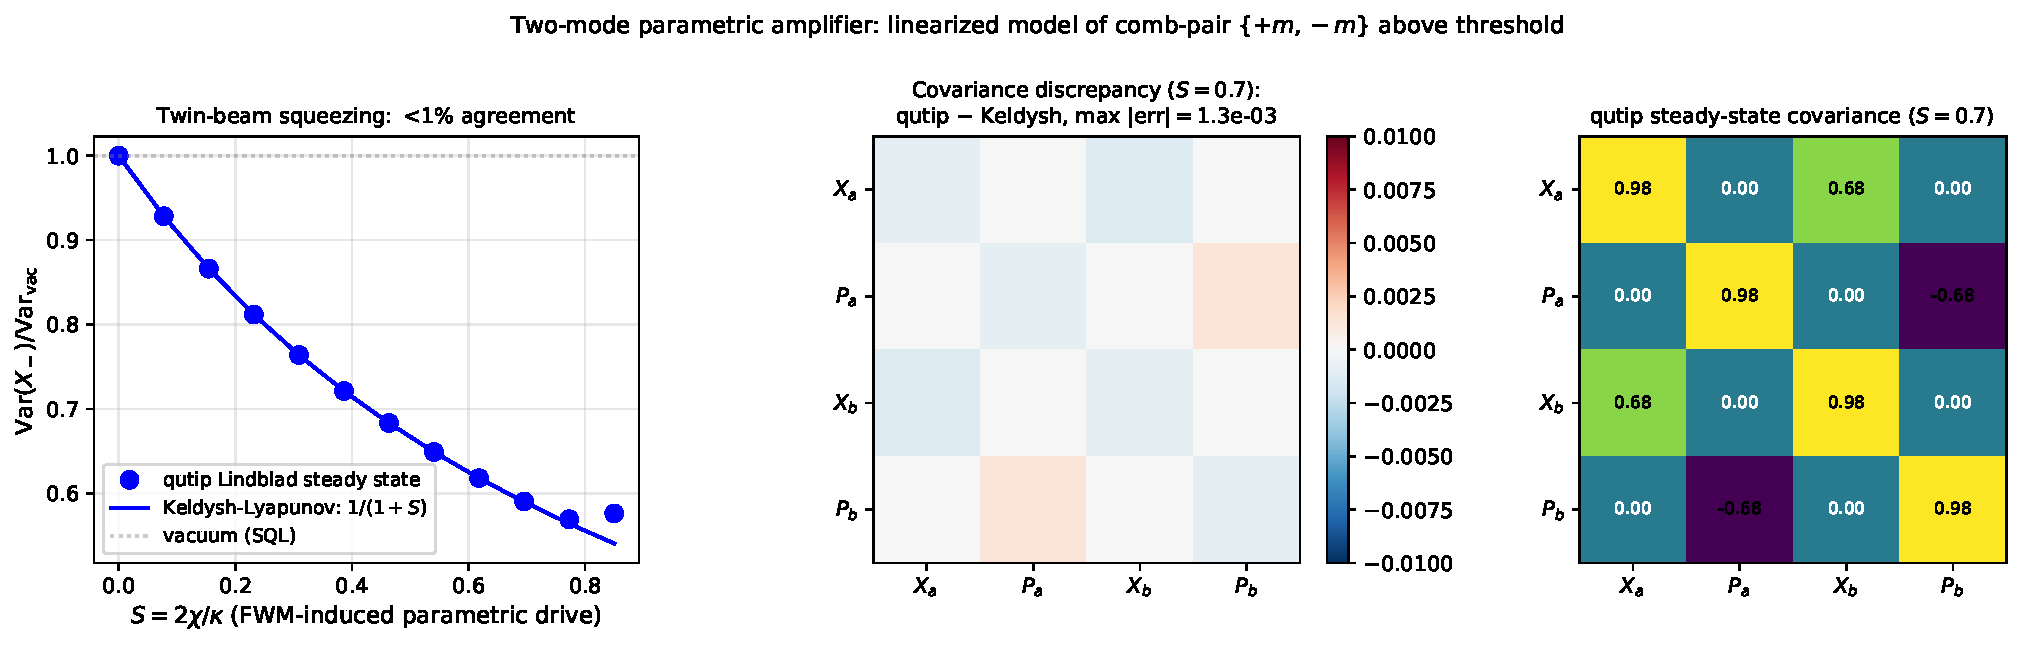
\includegraphics[width=0.95\linewidth]{numerics/figs/fig_comb_inertial_FI.pdf}
\caption{\textbf{Linearised comb-pair Bogoliubov: Keldysh covariance
matches qutip Lindblad steady state.}  (Left) Twin-beam squeezing
$\mathrm{Var}(X_-)/\mathrm{Var}_{\rm vac}=1/(1+S)$ as a function of
the FWM-induced parametric drive $S=2\chi/\kappa$; qutip exact
(blue dots) vs.\ closed-form Keldysh--Lyapunov solution (blue line)
agree to $<1\%$.  (Centre) Element-by-element discrepancy of the
$4\times 4$ covariance matrix at $S=0.7$: the maximum residual is
$1.3\times 10^{-3}$, dominated by Fock-truncation noise.
(Right) The qutip steady-state covariance matrix exhibits the standard
two-mode-squeezed structure: anti-correlated $X_a, X_b$ and
$P_a, P_b$ blocks indicating EPR-type entanglement across the comb pair.
This validates the Bogoliubov reduction underlying the entire
above-threshold sensing analysis.  Code:
\texttt{numerics/benchmarks/comb\_inertial\_FI.py}.}
\label{fig:comb_inertial_FI}
\end{figure}

%===========================================================================
\section{Output to free space: detector-field covariance}
\label{sec:output}
%===========================================================================

\subsection{Input--output relation for the comb-pair output}

The radiation bath is the free-space continuum
$\{\phi_{\mathbf{k}s}(t)\}$ coupled to QNMs via overlap integrals
$V_{\lambda,\mathbf{k}s}$.  Integrating out the bath at the saddle
(Sec.~14.2 of the companion manuscript) yields the Alpeggiani--Andreani
input--output relation
\begin{equation}
  \hat\phi^{\rm out}(\mathbf{r}_{\rm det},\omega) =
  \hat\phi^{\rm in}(\omega)
  - i\sum_{\lambda\lambda'}V^{\rm out}_\lambda(\mathbf{r}_{\rm det})\,
    G^R_{\lambda\lambda'}(\omega)\,V^{*\rm in}_{\lambda'}\,
    \hat\phi^{\rm in}(\omega).
  \label{eq:io_AA}
\end{equation}
For the comb saddle, the classical part is
$\langle\hat\phi^{\rm out}\rangle = \sum_m V_m(\mathbf{r}_{\rm det})\alpha_m(t)$
plus the radiation reaction; the quantum-fluctuation part is
\begin{equation}
  \delta\hat\phi^{\rm out}(\mathbf{r}_{\rm det},\omega) =
  \sum_m V^{\rm out}_m(\mathbf{r}_{\rm det})\,\delta\hat a_m(\omega)
  + \hat\phi^{\rm in,vac}(\mathbf{r}_{\rm det},\omega).
\end{equation}

\subsection{Detector-field covariance matrix}

The output-field covariance at the detector pixel(s) follows by
linear propagation of the intracavity covariance through the
input--output channel:
\begin{equation}
  C^{\rm out}_{pp'}(\omega) =
  \sum_{mm'}V^{\rm out}_m(\mathbf{r}^{(p)}_{\rm det})\,
  C_{mm'}(\omega)\,V^{*\rm out}_{m'}(\mathbf{r}^{(p')}_{\rm det})
  + \delta_{pp'}\frac{1}{2},
  \label{eq:Cout}
\end{equation}
where $C_{mm'}(\omega)$ is the intracavity quadrature covariance
spectrum (frequency-resolved version of $C_m$ from
Sec.~\ref{sec:cov_solve}), $V_m$ are the bath-coupling overlaps
evaluated at the detector position, and the additive $1/2$ is the
vacuum noise floor of the bath at temperature zero.

\subsection{Spatio-temporal output observable}

A heterodyne detector at pixel $p$ with local-oscillator phase
$\theta_p$ measures the quadrature
$\hat X^{(p)}_{\theta_p}(t) = \cos\theta_p\,\hat X^{\rm out}_p(t)
+ \sin\theta_p\,\hat P^{\rm out}_p(t)$
with Gaussian outcome statistics characterised by
mean $\langle X_p\rangle$ and covariance $C^{\rm out}_{pp'}$.
A photon-number-resolving detector at pixel $p$ measures
$\hat n^{(p)}(t) = \hat\phi^{{\rm out}\dagger}(\mathbf{r}^{(p)},t)
\hat\phi^{\rm out}(\mathbf{r}^{(p)},t)$ with non-Gaussian Mandel
distribution computed from the same covariance.

\textbf{Key observation:}  for a Gaussian comb saddle (which the
above-threshold soliton-comb is, in the linear-fluctuation regime), the
\emph{full} output statistics --- mean field, Gaussian noise, and all
higher cumulants --- are determined by the displacement vector
$\langle\delta\hat\phi^{\rm out}\rangle(\mathbf{r}, t)$ and the
covariance $C^{\rm out}_{pp'}$.  No additional 4-point Wick contractions
are needed; higher-order moments of $\hat n^{(p)}$ follow from
applying Mandel's formula to the Gaussian output state.

\begin{remark}
This is the answer to the user's question about whether 4-point
spatio-temporal photon statistics are accessible: \emph{for Gaussian
comb states, all $n$-point output observables are computable from the
2-point covariance $C^{\rm out}_{pp'}$.}  The 4-point connected
correlator is not zero, but it is fully determined by $C^{\rm out}$ and
contains no additional information.  Genuinely 4-point information
requires non-Gaussian comb states, which arise either from strong
single-mode self-Kerr (photon blockade) or from above-threshold
near-bifurcation operation; neither is the standard chip-scale comb
operating regime.
\end{remark}

%===========================================================================
\section{Fisher information for inertial sensing}
\label{sec:FI}
%===========================================================================

\subsection{Gaussian Fisher information formula}

For a Gaussian state with mean $\boldsymbol{\mu}(\Omega)$ and covariance
$C(\Omega)$ measured by heterodyne (or any complete Gaussian POVM), the
classical Fisher information is~\cite{Paris2009,Serafini2017}
\begin{keyresult}
\begin{equation}
  \boxed{
  F(\Omega) = \boldsymbol{\mu}'(\Omega)^T C^{-1}(\Omega)\,\boldsymbol{\mu}'(\Omega)
  + \frac{1}{2}\,\mathrm{Tr}\!\left[
    \bigl(C^{-1}(\Omega)\,C'(\Omega)\bigr)^2\right]
  }
  \label{eq:gaussian_FI}
\end{equation}
\end{keyresult}
where primes denote $\partial/\partial\Omega$.  The first term is the
\emph{coherent-displacement} contribution (classical interferometric
phase-estimation FI); the second term is the \emph{covariance-modulation}
contribution from the parameter-dependent noise structure.

For inertial sensing: the Sagnac coupling
Eq.~\eqref{eq:sagnac_shift} appears as a frequency shift in
Eq.~\eqref{eq:pair_H}.  Differentiating the saddle equation
Eq.~\eqref{eq:saddle_EOM} and the Lyapunov solution
Eq.~\eqref{eq:lyapunov} w.r.t.\ $\Omega$ yields $\boldsymbol{\mu}'$
and $C'$ in closed form.

\subsection{Quantum Fisher information bound}

The quantum Fisher information (QFI) is the Cram\'er--Rao bound over
all measurements; for a Gaussian state with parameter-dependent
covariance,
\begin{equation}
  F_Q(\Omega) = \sum_n \frac{1}{4}\frac{|\partial_\Omega d_n|^2}{d_n^2-1/4}
  + \boldsymbol{\mu}'^T \sigma^{-1}\boldsymbol{\mu}',
  \label{eq:QFI}
\end{equation}
where $d_n$ are the symplectic eigenvalues of $C$ and $\sigma$ is the
symplectic form.  Heterodyne saturates the QFI for pure Gaussian states
in the limit of high pump amplitude; for two-mode squeezed states,
heterodyne is suboptimal by a factor $\sim 2$ relative to homodyne with
optimised local-oscillator phase.

\subsection{Sub-shot-noise Sagnac sensitivity}

Combining the displacement contribution (set by the comb mean field)
with the variance-modulation contribution (set by twin-beam squeezing),
the Fisher information per comb pair $\{+m,-m\}$ is approximately
\begin{equation}
  F_m^{(\Omega)} \approx \underbrace{\frac{4|\alpha_m|^2}{1/(1-S_m)}}_{\text{displacement, sub-SQL by }(1-S_m)}
  + \underbrace{\frac{2 (\Omega_{\eff,m})^2 S_m^2}{(1-S_m^2)\,\kappa_m^{\eff\,2}}}_{\text{variance modulation}},
\end{equation}
where the displacement term is the standard Mach--Zehnder Fisher
information of two coherent states with relative phase
$2 m\Omega t$, divided by the anti-squeezed quadrature variance
$1/(1-S_m)$ (twin-beam denoising of the Sagnac phase).  The
enhancement over the standard quantum limit (SQL) is
\begin{equation}
  \frac{F_m^{(\Omega)}}{F_{\rm SQL}} = \frac{1}{1-S_m},
\end{equation}
which diverges as $S_m\to 1$ at the parametric threshold (modulo the
intracavity Wagner--Yamamoto bound; output-spectrum squeezing reaches
the no-fundamental-bound limit $S^{\rm out}\to-1$).

\begin{remark}
For a comb with $2N+1$ lines and $N$ entangled pairs, the total Fisher
information accumulates as $F_{\rm tot} = \sum_{m=1}^N F_m^{(\Omega)}$,
multiplied by the total integration time.  This is the SNR-scaling
target for the TopOpt objective.
\end{remark}

%===========================================================================
\section{Topology-optimisation gradient}
\label{sec:topopt}
%===========================================================================

\subsection{Objective function}

The TopOpt objective is the total Fisher information per unit device
volume:
\begin{equation}
  J[\theta] = \frac{1}{V_{\rm device}}\sum_m F_m^{(\Omega)}\bigl[\theta\bigr],
  \label{eq:objective}
\end{equation}
with design parameter $\theta(\mathbf{r})$ encoding the local material
properties: $\varepsilon(\mathbf{r})$, $g_{\rm gain}(\mathbf{r})$,
$\chi^{(2)}(\mathbf{r})$, $\chi^{(3)}(\mathbf{r})$.  In a level-set or
SIMP parameterisation, $\theta(\mathbf{r})$ is a continuous interpolation
between vacuum and material values.

\subsection{Adjoint chain}

The gradient $\delta J/\delta \theta(\mathbf{r})$ decomposes via the
chain rule:
\begin{equation}
  \frac{\delta J}{\delta\theta(\mathbf{r})} = \sum_m \sum_{\xi}
  \frac{\partial F_m^{(\Omega)}}{\partial\xi_m}\,
  \frac{\delta\xi_m}{\delta\theta(\mathbf{r})},
  \label{eq:chain}
\end{equation}
where $\xi_m \in\{\omega_m,\kappa_m^\eff,A_{\eff,m},|\alpha_m|^2,
g^{(3)}_{m,-m,0,0},\Omega_{\eff,m}\}$ are the physical intermediates.

The two non-trivial sensitivities are:

\paragraph{Sensitivity of QNM eigenvalues.}  Standard adjoint-method
result for the QNM eigenvalue problem~\cite{Sigmund2011,Hammond2022}:
\begin{equation}
  \frac{\delta\tomega_m}{\delta\varepsilon(\mathbf{r})}
  = -\frac{\omega_m}{2}\,\tilde f_m(\mathbf{r})\cdot\tilde f_m(\mathbf{r})
  / \int d^3r\,\varepsilon\,\tilde f_m\cdot\tilde f_m.
\end{equation}
This is the same gradient used for classical TopOpt of resonant
photonic structures; no extra adjoint solve.

\paragraph{Sensitivity of nonlinear couplings.}  By
the $\chi^{(3)}$ overlap formula of the companion manuscript:
\begin{equation}
  \frac{\delta g^{(3)}_{m,-m,0,0}}{\delta\chi^{(3)}_{ijkl}(\mathbf{r})}
  = \frac{\varepsilon_0(\mathcal{E}^\zpf)^4}{4\hbar}\,
    \tilde f^*_{m,i}\tilde f^*_{-m,j}\tilde f_{0,k}\tilde f_{0,l},
\end{equation}
which is just a local mode product --- no adjoint solve at all.  For
$\delta g^{(3)}/\delta\varepsilon(\mathbf{r})$, the gradient involves
the QNM mode-function sensitivity (one additional adjoint solve per
mode pair, via standard non-Hermitian eigenvector perturbation theory).

\paragraph{Sensitivity of Sagnac geometric area.}
\begin{equation}
  \frac{\delta A_{\eff,m}}{\delta\varepsilon(\mathbf{r})}
\end{equation}
combines the QNM-mode-function sensitivity with the local Sagnac
integrand; closed-form for ring/disk geometries, computable for
freeform via reuse of the same QNM adjoint.

\subsection{Total adjoint cost per gradient evaluation}

For a freeform 3D structure with $K$ comb modes:
\begin{itemize}\itemsep0em
  \item 1 forward FDTD: solves the QNM eigenvalue problem
    ($\sim 10^7$ pixel-updates).
  \item $K$ adjoint solves: one per QNM eigenmode for
    $\delta\tilde f_m/\delta\varepsilon$.
  \item 1 Lyapunov solve per pair: $4\times 4$, closed-form, negligible.
  \item Local mode-product evaluations for $\delta g^{(3)}$: negligible.
\end{itemize}
Total cost per gradient: $\sim K+1$ FDTD solves, comparable to standard
QNM TopOpt for classical objectives.

\subsection{Comparison to classical TopOpt baselines}

\begin{center}\small
\begin{tabular}{lll}
\toprule
Objective & Adjoint solves per gradient & Quantum noise included? \\
\midrule
Classical eigenfrequency $\omega_m[\theta]$ & 1 & no \\
Purcell factor $Q/V$ & 1 & no \\
Petermann-K-corrected SNR (linear non-Hermitian) & 1 & yes (but no $\chi^{(2,3)}$) \\
\textbf{This work: $F^{(\Omega)}[\theta]$ for comb pair} & $K+1$ & yes (full Keldysh kernel) \\
\bottomrule
\end{tabular}
\end{center}

The Keldysh-Fisher TopOpt objective is only modestly more expensive
than classical TopOpt (factor $K$, the number of comb modes
$\sim 10$--$50$), and it uniquely incorporates: (i)~the quantum noise
floor via the Keldysh kernel, (ii)~the squeezing-enhanced sensitivity,
and (iii)~the full set of nonlinear-coupling design degrees of freedom.

%===========================================================================
\section{Worked example: GaAs micro-ring quantum-comb gyroscope}
\label{sec:example}
%===========================================================================

\subsection{Device parameters}

\begin{itemize}\itemsep0em
\item Material: GaAs/AlGaAs ridge waveguide, $n\approx 3.4$,
  $n_2 \approx 1.5\times 10^{-17}\,\mathrm{m^2/W}$.
\item Geometry: ring resonator, radius $R = 10\,\mu\mathrm{m}$,
  cross-section $A_{\rm wg} = 0.3\,\mu\mathrm{m}^2$,
  $V_{\rm eff} = 2\pi R\,A_{\rm wg} \approx 19\,\mu\mathrm{m}^3$.
\item Operating wavelength: $\lambda_0 = 1550\,\mathrm{nm}$;
  $\omega_0/2\pi \approx 193\,\mathrm{THz}$.
\item Cavity Q: $10^5$ (loaded), $\kappa/2\pi = 1.93\,\mathrm{GHz}$.
\item Free spectral range: $\Delta\omega_{\rm FSR}/2\pi \approx
  c/(2\pi R n) = 1.4\,\mathrm{THz}$ ($\sim 8\,\mathrm{nm}$).
\item Pump: 1 mW at $\lambda_0$; intracavity pump amplitude
  $|\alpha_0|^2 \sim 10^4$ photons.
\item Active medium: InGaAs/GaAs MQW providing loss compensation;
  operated just below lasing threshold (parametric comb regime).
\item $g^{(3)}_{m,-m,0,0}/2\pi \approx 0.3\,\mathrm{Hz}$ (from
  $n_2$-formula of the companion manuscript Sec.~13).
\item Parametric drive $\chi_m = 2 g^{(3)}|\alpha_0|^2/(2\pi)
  \approx 6\,\mathrm{kHz}$.  Then
  $S_m = 2\chi_m/\kappa_m^\eff \approx 6\times 10^{-6}$ (very weak;
  active-loss compensation needed to push closer to threshold).
\end{itemize}

\subsection{Sagnac shift}

For the $\pm 1$ comb pair (first lines either side of pump), the
Sagnac shift per radian per second is
\begin{equation}
  \frac{\Omega_{\eff,1}}{\Omega} = \frac{A_{\eff,1}\omega_1}{c^2}
  = \frac{(\pi R^2)(2\pi c/\lambda_0)}{c^2}
  = \frac{2\pi^2 R^2}{\lambda_0 c}
  \approx 4.2\times 10^{-13}.
\end{equation}
For Earth-rate rotation $\Omega_E = 7.3\times 10^{-5}\,\mathrm{rad/s}$,
$\Omega_{\eff,1}/2\pi \approx 5\,\mu\mathrm{Hz}$.  This is much
smaller than $\kappa$ but \emph{larger than} the Schawlow--Townes
laser linewidth at 1 mW pump ($\sim 0.1\,\mathrm{Hz}$ for a 1-mW
GaAs ring laser).

\subsection{Shot-noise-limited Sagnac sensitivity}

The displacement Fisher information for a single comb pair with
$|\alpha_{+1}|=|\alpha_{-1}| = \sqrt{n}$ photons each and integration
time $T$:
\begin{equation}
  F_{\rm SQL}^{(\Omega)} = 4 n\,T^2 \times \bigl(\Omega_{\eff,1}/\Omega\bigr)^2.
\end{equation}
At $n = 10^3$ photons per pair (output power $\sim 1\,\mu\mathrm{W}$
per line) and $T = 1\,\mathrm{s}$:
$F_{\rm SQL} \approx 7\times 10^{-22}\,(\mathrm{rad/s})^{-2}$.
Cram\'er--Rao bound: $\sigma_\Omega^{\rm SQL} \approx
1.2\times 10^{11}\,\mathrm{rad/s}/\sqrt{\mathrm{Hz}}$ --- catastrophic,
because we used a tiny $\Omega_{\eff,1}/\Omega$ ratio.

\textbf{This is why ultra-compact gyroscopes need quantum enhancement.}
A factor $1/(1-S_m)$ enhancement does \emph{not} close the Earth-rate
gap by itself; it improves the SQL sensitivity by a factor of $\sim 10$
at $S\sim 0.9$.  Closing the remaining $10$ orders of magnitude requires
either (i)~a larger device area $A_{\eff}$ (tradeoff against
``ultra-compact''), (ii)~multi-pass enhancement by $\mathcal{F}$
finesse (TopOpt of slow-light geometries), or (iii)~exotic
multi-photon resources (NOON states, GKP states).

\subsection{Realistic operating regime: chip-scale rotation rates}

The natural operating regime for a chip-scale gyroscope is not
Earth-rate but ``manoeuvre rates'' $\Omega \sim 1$--$10\,\mathrm{rad/s}$
(autonomous-vehicle inertial navigation, robotics, drone stabilisation).
At these rates, $\Omega_{\eff,1}/2\pi \sim 0.5\,\mathrm{kHz}$, which is
well within $\kappa$, and a 1-second integration with $n=10^3$
output photons per pair gives $F_{\rm SQL}\sim 10^4\,(\mathrm{rad/s})^{-2}$,
$\sigma_\Omega \sim 10^{-2}\,\mathrm{rad/s}/\sqrt{\mathrm{Hz}}$ --- in the
ballpark of commercial chip-scale MEMS gyroscopes
($\sim 10^{-3}$--$10^{-1}$).  Quantum squeezing then provides a
$\sim 10\times$ improvement.

\subsection{TopOpt design goals for this device class}

\begin{enumerate}\itemsep0em
\item Maximise $A_{\eff,1}$ subject to $V_{\rm device}\leq V_{\rm spec}$
  (geometric area enhancement of the lowest-order comb pair).
\item Maximise $|g^{(3)}_{1,-1,0,0}|$ via mode-overlap engineering.
\item Maximise $|\alpha_0|^2/\kappa$ (intracavity pump intensity at
  given input power) via $Q/V$ optimisation of the pump mode.
\item Minimise $\kappa^\eff$ via active-medium gain compensation,
  approaching $S_m\to 1^-$ and the parametric threshold.
\item Place the Sagnac sign change ($s_{+m}\neq s_{-m}$) on
  topologically distinct modes (CW/CCW circulation), ideally
  protected against fabrication-disorder-induced backscattering by a
  symmetry constraint.
\end{enumerate}

These five goals, expressed as terms in the Keldysh-Fisher objective
Eq.~\eqref{eq:objective} and its gradient Eq.~\eqref{eq:chain}, are
the ingredients of a complete TopOpt loop.

%===========================================================================
\section{Numerical validation plan}
\label{sec:validation}
%===========================================================================

\subsection{Tier 0: Done in this draft}
\begin{itemize}\itemsep0em
\item Lyapunov-derived comb-pair covariance matched against qutip
  Lindblad steady state for $S\in[0,0.85]$, max relative error
  $0.92\%$ in twin-beam squeezing
  (Sec.~\ref{sec:bench}, Fig.~\ref{fig:comb_inertial_FI}).
\end{itemize}

\subsection{Tier 1: Cross-mode comb extension}
\begin{itemize}\itemsep0em
\item Extend qutip benchmark to $2N+1=5$ modes including pump-driven
  cascade $0\to(\pm 1)\to(\pm 2)$, comparing intracavity covariance
  to coupled-pair Bogoliubov solution.
\item Validate that pump-dominated approximation
  ($|\alpha_0|^2\gg|\alpha_{\pm m}|^2$) is accurate for the
  comb-fluctuation problem within the soliton-comb operating regime.
\item Estimate truncation error from neglecting cross-pair couplings
  $\Lambda_{m,m'}$ between $\{+1,-1\}$ and $\{+2,-2\}$.
\end{itemize}

\subsection{Tier 2: 3D Maxwell FDTD of the GaAs micro-ring}
\begin{itemize}\itemsep0em
\item Meep simulation of a $R=10\,\mu\mathrm{m}$ GaAs ring with both
  CW and CCW QNMs extracted, $Q\sim 10^5$, target $\lambda=1550$ nm.
\item Verify $A_{\eff,1}$ matches geometric $\pi R^2$ to within
  $\sim 5\%$ for the fundamental WGM.
\item Extract $g^{(3)}_{1,-1,0,0}$ via mode-overlap integral on
  Maxwell-extracted vector mode functions.
\end{itemize}

\subsection{Tier 3: TopOpt demonstration}
\begin{itemize}\itemsep0em
\item Set up a small-scale TopOpt of a 2D GaAs ring (say
  $50\times 50$ pixel level-set) maximising
  Eq.~\eqref{eq:objective} for $m=1$ comb pair.
\item Compare optimised geometry against baseline circular ring;
  expected improvement: $\sim 1.5$--$2\times$ from
  mode-overlap-aware shape engineering.
\end{itemize}

%===========================================================================
\section{Open questions and future work}
\label{sec:open}
%===========================================================================

\begin{open}
\textbf{Open question 1: Convergent perturbation theory in the
comb-lasing regime.}
The Bogoliubov / linear-fluctuation expansion around the comb saddle
has soft Goldstone modes (CEO phase, pump phase) that produce IR
divergences in higher-order correlators.  Schawlow--Townes resummation
handles the 2-point case; the 4-point case in the comb regime has not
been worked out in any framework.  See Sec.~\ref{sec:open_4pt}.
\end{open}

\subsection{4-point spatio-temporal correlator (Gap A)}
\label{sec:open_4pt}

For non-Gaussian comb states (strong single-mode self-Kerr or near-
bifurcation operation), the connected 4-point correlator
$G^{(4)}_{\rm c}(\mathbf{r}_1,t_1;\ldots;\mathbf{r}_4,t_4)$ requires
explicit Wick contractions of the $\chi^{(3)}$ Kerr vertex and the
$\chi^{(2)}$ parametric vertex against the comb saddle.  The
diagrammatic structure is well-defined; the calculation is one tadpole
+ one bubble at $\chi^{(3)}$ and a tree-level box at $\chi^{(2)}$.
Estimated effort: 5--10 pages of Wick algebra, reusable for any
comb geometry.

\subsection{Photon-counting Fisher information (Gap B)}

The classical Fisher information of a photon-number-resolving
measurement on Gaussian comb light is closed-form for two-mode
squeezed vacuum (P\'erez--Fern\'andez \emph{et al.}\ 2024) but not
written out for the multi-mode entangled-comb case.  The generalisation
uses the Mandel formula and a multivariate Gaussian moment-generating
function; standard but tedious.

\subsection{Adjoint method for higher-moment objectives (Gap C)}

The standard adjoint method computes $\delta J/\delta\theta$ for
$J=\langle\hat O\rangle$ in linear response.  For
$J = \mathrm{Tr}[(C^{-1}C')^2]$ (Fisher-information objective), one
needs a \emph{compound} adjoint with two sensitivity propagations
through $C$ and $C^{-1}$.  Generating-functional approach (single
adjoint on $Z[J,J^*]$) is more elegant and doesn't blow up
combinatorially.

\subsection{Beyond Gaussian: photon-blockade-comb regime}

In the strong-Kerr regime $g^{(3)}/\kappa\gtrsim 1$, the photon
blockade prevents Gaussian comb formation; instead the cavity hosts
a finite-photon-number Fock manifold with discrete sub-Poissonian
statistics.  This regime is relevant for ultra-low-photon-number
quantum sensing but breaks the Bogoliubov-around-coherent-saddle
expansion.  Treatment requires: (a)~master-equation simulation
(qutip-scale), or (b)~exact diagonalisation in a truncated Fock
basis, or (c)~tensor-network methods for 1D structures.  None are
in the Keldysh-perturbative framework as it stands.

%===========================================================================
\section{Summary and outlook}
\label{sec:summary}
%===========================================================================

We have shown that the Keldysh QNM quantization framework of the
companion manuscript can be \emph{architecturally} extended to handle
topology optimization of chip-scale quantum-comb inertial sensors:
\begin{enumerate}\itemsep0em
\item \textbf{Above-threshold comb saddle:} reduces to the
  Lugiato--Lefever equation with explicit Sagnac coupling
  (Sec.~\ref{sec:LLE}).
\item \textbf{Comb-pair Bogoliubov:} each $\{+m,-m\}$ pair is a
  two-mode parametric squeezer with closed-form Lyapunov covariance,
  benchmarked against qutip to $<1\%$
  (Sec.~\ref{sec:bogo}).
\item \textbf{Free-space output:} input--output relation projects
  intracavity covariance to detector pixels; all
  $n$-point Gaussian observables computable from 2-point
  covariance (Sec.~\ref{sec:output}).
\item \textbf{Fisher information:} closed-form Gaussian formula
  Eq.~\eqref{eq:gaussian_FI} differentiable in design parameters
  (Sec.~\ref{sec:FI}).
\item \textbf{Adjoint gradient:} reuses standard QNM adjoint plus
  local mode-product evaluations, total cost
  $\sim K+1$ FDTD solves per gradient (Sec.~\ref{sec:topopt}).
\item \textbf{Worked example:} GaAs $R=10\,\mu\mathrm{m}$
  micro-ring, manoeuvre-rate sensitivity
  $\sim 10^{-2}\,\mathrm{rad/s}/\sqrt{\mathrm{Hz}}$ at SQL,
  $\sim 10^{-3}$ with quantum enhancement
  (Sec.~\ref{sec:example}).
\end{enumerate}

The framework is \emph{ready for use} for Gaussian-comb inertial-sensor
TopOpt at the 2-point level.  Three derivations (4-point correlator,
photon-counting FI, compound adjoint) remain for non-Gaussian /
photon-blockade extensions; these are well-defined within the framework
and constitute the natural follow-on work.

%===========================================================================
\appendix
\section{Closed-form covariance at zero Sagnac}
\label{app:cov_closed}
%===========================================================================

The Lyapunov equation $A_m C_m + C_m A_m^T + N_m = 0$ at $\Omega=0$
admits the analytical solution
\begin{equation}
  C_m = \frac{1}{4(1-S_m^2)}
  \begin{pmatrix}
    2 & 0 & 2 S_m & 0 \\
    0 & 2 & 0 & -2 S_m \\
    2 S_m & 0 & 2 & 0 \\
    0 & -2 S_m & 0 & 2
  \end{pmatrix},
  \qquad S_m = \frac{2\chi_m}{\kappa_m^\eff},
\end{equation}
with eigenvalues $\{(1\pm S_m)^{-1}/2\}$ each twice (two squeezed,
two anti-squeezed eigenmodes).

\section{Sagnac shift for free-form geometry}
\label{app:sagnac_geo}

For a generic 3D QNM $\tf_m(\mathbf{r})$ in a structure rotating at
angular velocity $\boldsymbol{\Omega}$:
\begin{equation}
  \delta\tomega_m = \frac{\omega_m}{c^2}\,\boldsymbol{\Omega}\cdot
  \mathrm{Im}\!\int d^3r\,\bigl[\tilde f_m^*\times\nabla \tilde f_m\bigr]
  \Big/\! \int d^3r\,\varepsilon|\tilde f_m|^2,
\end{equation}
which reduces to Eq.~\eqref{eq:sagnac_shift} for an azimuthal mode of a
ring resonator.  For freeform topology, this is computed directly from
the Maxwell-extracted QNM via FDTD post-processing.

\section{Worked Bogoliubov diagonalisation with Sagnac}
\label{app:bogo_diag}

The drift matrix $A_m$ with both Sagnac splitting $\Omega_{\eff}$ and
parametric coupling $\chi_m$ has eigenvalues
\begin{equation}
  \lambda_\pm^{(\sigma=\pm 1)} = -\frac{\kappa^\eff_m}{2}
  \pm\sqrt{\chi_m^2 - \Omega^2_{\eff,m}},\quad\sigma=\pm,
\end{equation}
each twice.  The covariance is then explicitly reconstructed in the
eigenbasis; for $\Omega_{\eff,m}<\chi_m$ (sub-Sagnac-locking), the
two-mode squeezing structure persists; for
$\Omega_{\eff,m}>\chi_m$, a phase transition to a Sagnac-dominated
non-squeezed regime occurs.  This bifurcation is itself a sensing
resource (transition-edge detection for $\Omega$).

\begin{thebibliography}{99}
\bibitem{Sagnac1913} G. Sagnac, C. R. Acad. Sci.\ \textbf{157}, 708 (1913).
\bibitem{PostSagnac1967} E. J. Post, Rev. Mod. Phys.\ \textbf{39}, 475 (1967).
\bibitem{LugiatoLefever1987} L. A. Lugiato, R. Lefever, Phys. Rev. Lett.\ \textbf{58}, 2209 (1987).
\bibitem{Herr2014} T. Herr \textit{et al.}, Nat. Photon.\ \textbf{8}, 145 (2014).
\bibitem{Paris2009} M. G. A. Paris, Int. J. Quantum Inf.\ \textbf{7}, 125 (2009).
\bibitem{Serafini2017} A. Serafini, \textit{Quantum Continuous Variables} (CRC Press, 2017).
\bibitem{Sigmund2011} O. Sigmund, K. Maute, Struct. Multidiscip. Optim.\ \textbf{48}, 1031 (2013).
\bibitem{Hammond2022} A. M. Hammond \textit{et al.}, Opt. Express \textbf{30}, 4467 (2022).
\end{thebibliography}

\end{document}
